\documentclass[11pt,a4paper]{article}
\usepackage[margin=2.2cm]{geometry}
\usepackage[T1]{fontenc}
\usepackage{lmodern}
\usepackage{microtype}
\usepackage{amsmath,amssymb}
\usepackage{booktabs,tabularx,multirow,xltabular}
\usepackage{xcolor}
\usepackage{enumitem}
\usepackage{caption}
\usepackage{float}
\usepackage[section]{placeins}
\usepackage{needspace}
\usepackage{etoolbox}
\pretocmd{\section}{\needspace{10\baselineskip}}{}{}
\usepackage{tikz}
\usetikzlibrary{arrows.meta,positioning,fit,calc}
\usepackage{pgfplots}
\pgfplotsset{compat=1.18}
\usepackage[colorlinks=true,linkcolor=blue!50!black,citecolor=blue!50!black,urlcolor=blue!50!black]{hyperref}
\newcolumntype{Y}{>{\raggedright\arraybackslash}X}
\newcolumntype{P}[1]{>{\raggedright\arraybackslash}p{#1}}
\newcommand{\pzf}{$\pi_{0.5}$}
\newcommand{\pzs}{$\pi_{0.7}$}
\definecolor{cA}{HTML}{4C72B0}
\definecolor{cB}{HTML}{DD8452}
\definecolor{cC}{HTML}{55A868}
\definecolor{cD}{HTML}{C44E52}
\definecolor{cE}{HTML}{8172B3}
\definecolor{cG}{HTML}{999999}
\setlist{itemsep=2pt,topsep=3pt,leftmargin=*}
\captionsetup{font=small,labelfont=bf}
\renewcommand{\arraystretch}{1.2}
\setlength{\parskip}{4pt}
\setlength{\parindent}{0pt}
% figures and tables may share pages with text; float-only pages stack from the top
\renewcommand{\topfraction}{0.9}\renewcommand{\bottomfraction}{0.8}\renewcommand{\textfraction}{0.07}
\renewcommand{\floatpagefraction}{0.8}\setcounter{topnumber}{3}\setcounter{bottomnumber}{2}\setcounter{totalnumber}{5}
\makeatletter\setlength{\@fptop}{0pt}\setlength{\@fpsep}{14pt plus 2pt}\setlength{\@fpbot}{0pt plus 1fil}\makeatother
\newcommand{\sub}[1]{\par\needspace{4\baselineskip}\smallskip\noindent\textbf{#1}\par}
\newcommand{\parttitle}[1]{\clearpage\begin{center}{\Large\bfseries #1}\end{center}\vspace{2mm}}
\pgfplotsset{every axis/.append style={font=\small, ymajorgrids, grid style={gray!25}, axis lines*=left,
  nodes near coords, nodes near coords style={font=\scriptsize}, ymin=0,
  legend style={font=\scriptsize, draw=none, fill=none, at={(0.5,-0.22)}, anchor=north, legend columns=-1, /tikz/every even column/.append style={column sep=6pt}}}}

\begin{document}
\begin{center}
{\LARGE\bfseries Robot stack for OpenArm~2}\\[4pt]
{\large Experiments, insights and proposal}\\[4pt]
{\small 26 October 2026}
\end{center}

\section*{Summary}
\sub{Insights from the experiments}
\begin{enumerate}[label=\textbf{\arabic*.}]
\item The motion expert executes its first command well, but rarely follows a change of instruction and keeps no memory of earlier steps.
\item A trained noise policy makes the robot follow a change of instruction twice as often, with no target point and no change to the motion expert. Stopping, setting down, retracting and re-commanding is the most reliable redirect inside full missions.
\item A world model helps at the level of subtasks, not motions: imagining the outcome of each subtask lets the robot reach goals shown as a photo and complete far more missions.
\item Memory works outside the motion expert: an activity log for interruptions, rules for standing instructions, counters for what the camera cannot see.
\item Qwen3-VL-4B is the stronger of the two planners tested; picture goals and standing instructions need the world model and rules memory.
\end{enumerate}

\sub{Proposal}
\begin{enumerate}[label=\textbf{\arabic*.}]
\item \textbf{Motion expert}: LingBot-VLA 2.0, compared with \pzf\ and GR00T in simulation and on the OpenArm~2 data.
\item \textbf{Steering}: the noise policy as the learned steering module, with stop--set down--retract as the fallback.
\item \textbf{World model}: beside the planner, imagining the outcome of each candidate subtask.
\item \textbf{Memory}: activity log, rules, counters, video memory and a progress monitor.
\item \textbf{Planner}: Qwen3-VL-4B as the baseline; fine-tuned and larger planners to evaluate.
\item \textbf{Data and training}: one flywheel where the robot's logs train every module.
\end{enumerate}

%==================================================================
\parttitle{Part I \quad Experiments and insights}

\section{The motion expert}
\label{sec:vla}
\sub{G0.5 in our tests}
\begin{itemize}
\item \textbf{Fixed commands}: on LIBERO, a set of simulated tabletop tasks, it succeeds 97--99\% of the time when the instruction stays the same.
\item \textbf{Change of instruction}: when the instruction changes 2\,s into a task, it completes the new task only 13--29\% of the time (\S\ref{sec:steer}).
\item \textbf{No memory}: it acts on the current camera frame only; when the instruction is removed after 2\,s, success falls to 40\% (\S\ref{sec:mem}).
\end{itemize}

\begin{figure}[!htbp]\centering
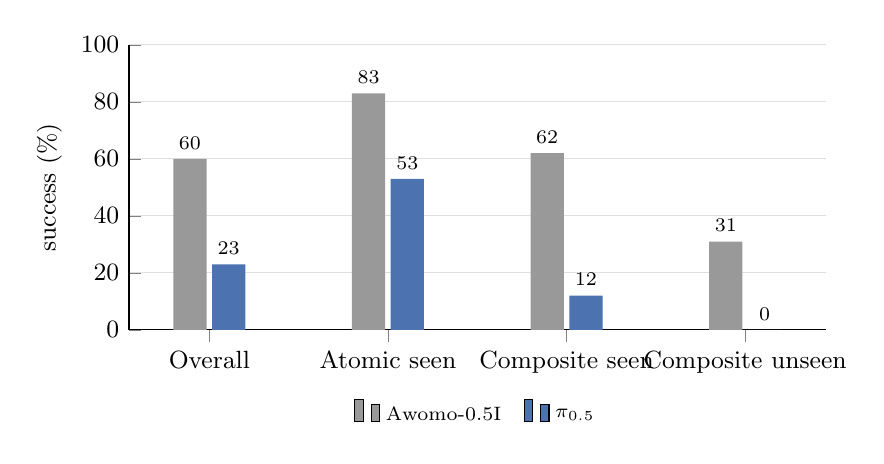
\begin{tikzpicture}
\begin{axis}[ybar, bar width=12pt, width=0.86\textwidth, height=5.2cm, ymax=100, ylabel={success (\%)}, enlarge x limits=0.15,
  symbolic x coords={Overall,Atomic seen,Composite seen,Composite unseen}, xtick=data]
\addplot[fill=cG, draw=none] coordinates {(Overall,60) (Atomic seen,83) (Composite seen,62) (Composite unseen,31)};
\addplot[fill=cA, draw=none] coordinates {(Overall,23) (Atomic seen,53) (Composite seen,12) (Composite unseen,0)};
\legend{{Awomo-0.5I}, {\pzf}}
\end{axis}
\end{tikzpicture}
\caption{RoboCasa365 kitchen benchmark, 50 tasks $\times$ 2 trials. ``Atomic'': one skill; ``composite'': several skills chained; ``unseen'': not in training.}
\label{fig:rc365}
\end{figure}

\sub{Benchmark}
\begin{itemize}
\item On the same 50 kitchen tasks, Awomo-0.5I succeeds 60\% of the time and \pzf\ 23\%: the choice of motion expert matters.
\item Composite tasks are the hardest, unseen ones most of all (31\% and 0\%).
\end{itemize}

\sub{Insights}
\begin{itemize}
\item The motion expert is reliable on short, fixed commands.
\item Changing tasks, remembering and chaining long tasks need modules around it: steering, memory and a planner that splits work into short subtasks.
\end{itemize}

\sub{What the literature shows}
G0.5~\cite{g05} reaches 98.9\% on LIBERO. \pzf~\cite{pi05} and \pzs~\cite{pi07} pair a VLM with a flow-matching action expert and take subtask instructions from a high level. Awomo-0.5I~\cite{awomo} is a strong RoboCasa365~\cite{robocasa365} policy.

%==================================================================
\section{Steering: changing the task mid-motion}
\label{sec:steer}
\sub{The problem}
The robot is reaching for the bowl and the user says ``no, the bottle''. A motion expert keeps doing its first task.

\sub{The idea: a noise policy}
The motion expert turns random noise into a motion. A small network that sees the cameras, the robot state and the new instruction chooses that noise, so the expert's own motion heads toward the new task. The expert itself is never modified. The network is trained in two stages:
\begin{enumerate}
\item imitate the noise of the robot's successful rollouts (DSBC);
\item improve it through a learned world model and a success critic, back-propagating through the expert's sampler (SuperMimic-style).
\end{enumerate}

\begin{figure}[!htbp]\centering
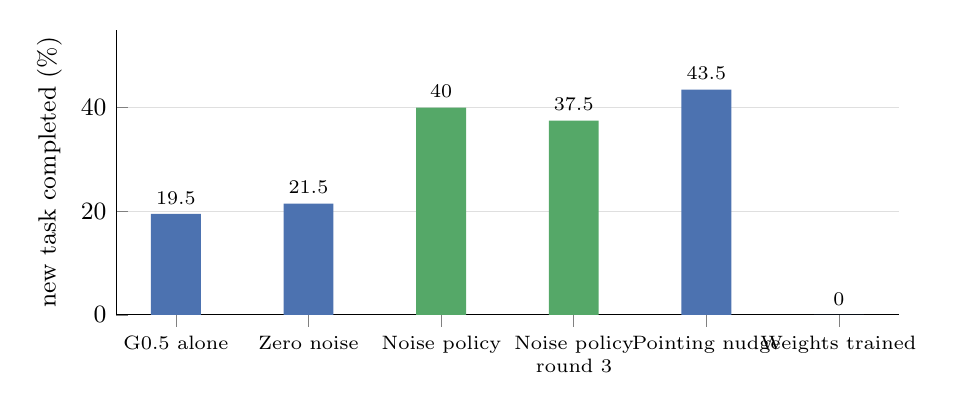
\begin{tikzpicture}
\begin{axis}[ybar, bar width=18pt, width=0.95\textwidth, height=5.2cm, ymax=55, ylabel={new task completed (\%)}, enlarge x limits=0.09,
  symbolic x coords={G0.5 alone,Zero noise,Noise policy,Noise policy round 3,Pointing nudge,Weights trained},
  xtick={G0.5 alone,Zero noise,Noise policy,Noise policy round 3,Pointing nudge,Weights trained},
  x tick label style={font=\scriptsize, align=center, text width=2.0cm}]
\addplot[fill=cA, draw=none, bar shift=0pt] coordinates {(G0.5 alone,19.5) (Zero noise,21.5) (Pointing nudge,43.5) (Weights trained,0)};
\addplot[fill=cC, draw=none, bar shift=0pt] coordinates {(Noise policy,40) (Noise policy round 3,37.5)};
\end{axis}
\end{tikzpicture}
\caption{Instruction changed after 2\,s; 200 trials per bar on start states not used for training.}
\label{fig:steer}
\end{figure}

\sub{Results: instruction changed after 2\,s}
\begin{itemize}
\item The noise policy completes \textbf{40\%} of new tasks, against 19.5\% for G0.5 alone.
\item This matches the pointing nudge (43.5\%), a 2\,s push toward the new target, without needing any target point.
\item Zero noise gives 21.5\%: the gain comes from what the policy sees.
\item A third training round with fresh data stays at the same level (37.5\%).
\item Training the expert's own weights with the same objective gives 0\% and also breaks its normal tasks.
\end{itemize}

\begin{table}[!htbp]\centering\small
\begin{tabularx}{\textwidth}{P{5.0cm}cccY}
\toprule
Method & Target point & Training & Changes the expert & Result \\
\midrule
Repeat the new command & no & no & no & 13--29\% \\
Pointing nudge (person or VLM) & yes & no & no & 39--49\% \\
\textbf{Noise policy} & \textbf{no} & per skill & \textbf{no} & \textbf{40\%} \\
Train the expert's weights & no & yes & yes & 0\% \\
Stop, set down, retract, re-command & no & no & no & 96\% in missions \\
\bottomrule
\end{tabularx}
\caption{Ways to redirect the motion expert.}
\end{table}

\begin{figure}[!htbp]\centering
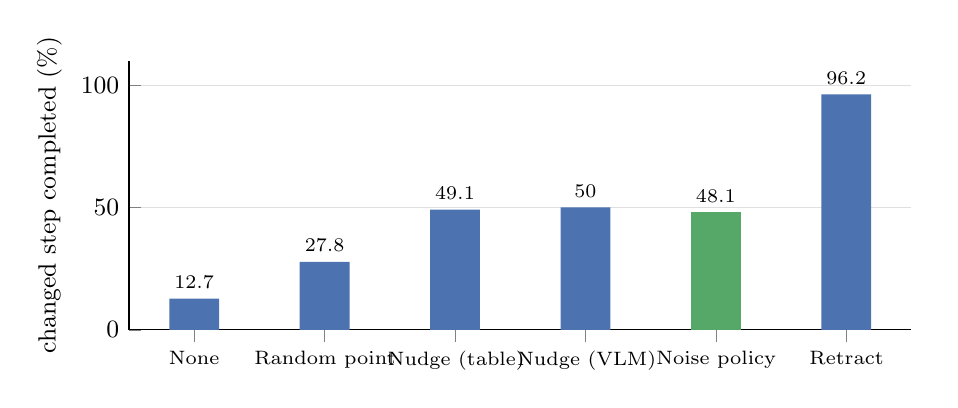
\begin{tikzpicture}
\begin{axis}[ybar, bar width=18pt, width=0.95\textwidth, height=5.0cm, ymax=110, ylabel={changed step completed (\%)}, enlarge x limits=0.1,
  symbolic x coords={None,Random point,Nudge (table),Nudge (VLM),Noise policy,Retract},
  xtick={None,Random point,Nudge (table),Nudge (VLM),Noise policy,Retract}, x tick label style={font=\scriptsize, align=center, text width=1.9cm}]
\addplot[fill=cA, draw=none, bar shift=0pt] coordinates {(None,12.7) (Random point,27.8) (Nudge (table),49.1) (Nudge (VLM),50.0) (Retract,96.2)};
\addplot[fill=cC, draw=none, bar shift=0pt] coordinates {(Noise policy,48.1)};
\end{axis}
\end{tikzpicture}
\caption{Change of mind inside full kitchen missions (``actually, don't do X, do Y''), about 53 missions per bar. \emph{Nudge (table)}: target from a per-task table; \emph{Nudge (VLM)}: the planner points at the target in the image; \emph{Retract}: back to the rest pose, then the new command.}
\label{fig:steermis}
\end{figure}

\sub{Results: inside full missions}
\begin{itemize}
\item Stop, retract and re-command completes 96\% of changed steps, the noise policy and the nudge about 50\%, no steering 13\%.
\item Targets pointed by a VLM, often 15\,cm off, work as well as exact ones; a random target does not.
\item When the change comes in the middle of a grasp, setting the object down before retracting keeps the success rate and places the object instead of dropping it (Table~\ref{tab:grasp}). No retraction touched the scene in $\approx$480 tries.
\end{itemize}

\begin{table}[!htbp]\centering\small
\begin{tabularx}{\textwidth}{YP{2.7cm}P{2.7cm}P{2.7cm}}
\toprule
Change of mind in the middle of a grasp & Changed step done & Holding an object at the change & Arm contacts per mission \\
\midrule
No steering & 8/67 & 2/12 & 3.0 \\
Retract, fingers open & 56/69 & 13/15 & 0.3 \\
Retract, keep the grasp & 48/69 & 8/16 & 0.0 \\
\textbf{Set down, then retract} & \textbf{54/67} & \textbf{11/13} & 1.0 \\
\bottomrule
\end{tabularx}
\caption{Retraction after a change of mind in the middle of a grasp.}
\label{tab:grasp}
\end{table}

\sub{Results: style preferences}
The same noise-and-guidance interface steers style. PrefPI raised the height at which the robot carries objects by 52\% at $\approx$90\% success; mixing original demonstrations into each round kept the policy from drifting.

\sub{Insights}
\begin{itemize}
\item A learned noise policy redirects the expert as well as pointing does, without a target and without touching the expert.
\item Changing the expert's weights against a learned critic breaks it; the noise is the safe place to steer.
\item Inside missions, a full retraction is the most reliable redirect; setting a held object down first keeps it safe.
\end{itemize}

\sub{What the literature shows}
Flow Reversal Steering~\cite{frs} steers a frozen flow policy from a rough reference and trains a noise policy on the successful noises. DSRL~\cite{dsrl} learns a noise policy with reinforcement learning on real robots, and FlowDAgger~\cite{flowdagger} with human corrections. SuperMimic~\cite{supermimic} trains a controller by back-propagating through one learned world model. Classifier-free guidance~\cite{cfg} works as a policy-improvement operator~\cite{cfgrl}; PrefPI~\cite{prefpi} uses it to steer style from a few labelled rollouts.

%==================================================================
\section{World model}
\label{sec:wm}
\sub{Roles tested}
\begin{itemize}
\item \textbf{Motion checker}: pick the best of several action chunks for the current command.
\item \textbf{Motion-level goal reading}: imagine 1.6\,s of motion for each command and keep the one closest to a goal photo.
\item \textbf{Subtask-level goal reading}: imagine the scene at the \emph{end} of each command and keep the one closest to the goal photo.
\item \textbf{Video prediction} on real household recordings (DROID).
\end{itemize}

\sub{How the subtask-level model works}
\begin{enumerate}
\item Encode the current camera view (DINOv3 features).
\item For each candidate command, predict the features of the scene at the end of that command.
\item Compare each prediction with the goal photo.
\item Run the command whose predicted end state is closest.
\end{enumerate}
It is trained on (start view, command $\rightarrow$ end view) pairs from demonstrations, in 3 minutes on a CPU.

\begin{figure}[!htbp]\centering
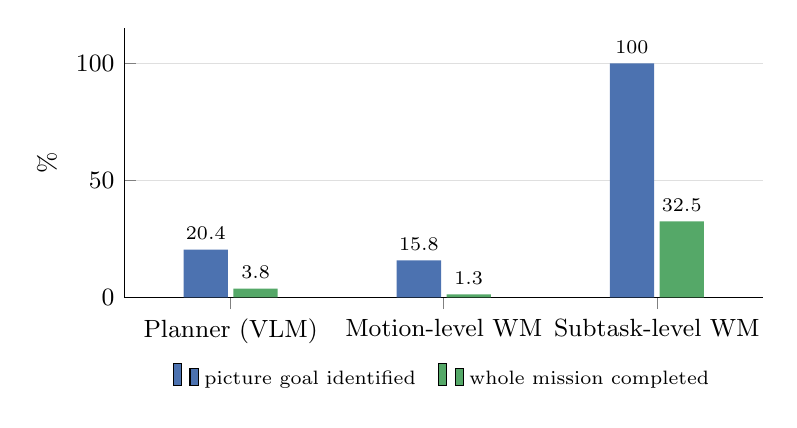
\begin{tikzpicture}
\begin{axis}[ybar, bar width=16pt, width=0.80\textwidth, height=5.0cm, ymax=115, ylabel={\%}, enlarge x limits=0.25,
  symbolic x coords={Planner (VLM),Motion-level WM,Subtask-level WM}, xtick=data]
\addplot[fill=cA, draw=none] coordinates {(Planner (VLM),20.4) (Motion-level WM,15.8) (Subtask-level WM,100)};
\addplot[fill=cC, draw=none] coordinates {(Planner (VLM),3.8) (Motion-level WM,1.3) (Subtask-level WM,32.5)};
\legend{picture goal identified, whole mission completed}
\end{axis}
\end{tikzpicture}
\caption{Picture-goal step of a three-step kitchen mission (``\ldots then make the kitchen look like this photo''), 80 missions per arm. The robot sees only its camera and the goal photo.}
\label{fig:wm}
\end{figure}

\sub{Results}
\begin{itemize}
\item The subtask-level model identifies \textbf{53/53} picture goals; the planner reading the photo identifies 11/54.
\item Whole missions completed: \textbf{26/80} with the subtask-level model, 3/80 with the planner.
\item Imagining only 1.6\,s of motion is not enough: ``turn on the stove'' and ``put the bowl on the stove'' look the same for the first second (right command 12\% of the time).
\item As a motion checker the world model adds nothing: the expert's alternatives for one command are nearly identical.
\end{itemize}

\begin{table}[!htbp]\centering\small
\begin{tabularx}{\textwidth}{P{4.4cm}Y}
\toprule
Role & Result \\
\midrule
Motion checker & 57 vs 56/80 steps; with diverse proposals, same as a random pick \\
Motion-level goal reading & right command 12\% of the time \\
\textbf{Subtask-level goal reading} & \textbf{53/53} goals, missions 3/80 $\rightarrow$ \textbf{26/80}; 97\% on held-out demonstrations \\
Critic and dynamics for steering & trains the noise policy (\S\ref{sec:steer}) \\
Household video prediction (DROID) & FLUX~3 Action best on folding (0.70$\times$ the error of holding still); RoboJEPA improves with size (0.81 $\rightarrow$ 0.66$\times$) and plans 4$\times$ faster with gradients \\
\bottomrule
\end{tabularx}
\caption{World-model results.}
\end{table}

\sub{Insights}
\begin{itemize}
\item The world model is useful at the level of subtasks: imagining what the scene looks like once a command is done.
\item At the level of motions it is not: short imagination cannot tell commands apart, and the expert's alternatives barely differ.
\end{itemize}

\sub{What the literature shows}
Latent world models predict future image features instead of pixels: LaWAM~\cite{lawam}, RoboJEPA~\cite{robojepa} and FLARE~\cite{flare}. World-action models such as Cosmos~3~\cite{cosmos3}, FLUX~3 Action~\cite{flux3a} and OpenWAM~\cite{openwam} predict video and actions together. DreamerV3~\cite{dreamerv3}, TD-MPC2~\cite{tdmpc2} and SuperMimic~\cite{supermimic} plan or learn inside such models.

%==================================================================
\section{Memory}
\label{sec:mem}
\begin{figure}[!htbp]\centering
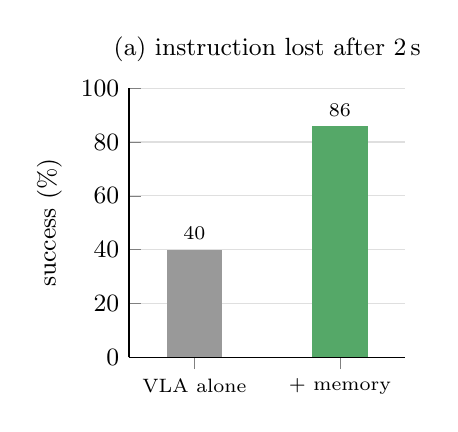
\begin{tikzpicture}
\begin{axis}[ybar, bar width=20pt, width=0.42\textwidth, height=5.0cm, ymax=100, ylabel={success (\%)}, enlarge x limits=0.45,
  symbolic x coords={VLA alone,+ memory}, xtick={VLA alone,+ memory}, x tick label style={font=\scriptsize}, title={\small (a) instruction lost after 2\,s}]
\addplot[fill=cG, draw=none, bar shift=0pt] coordinates {(VLA alone,40)};
\addplot[fill=cC, draw=none, bar shift=0pt] coordinates {(+ memory,86)};
\end{axis}
\end{tikzpicture}\hfill
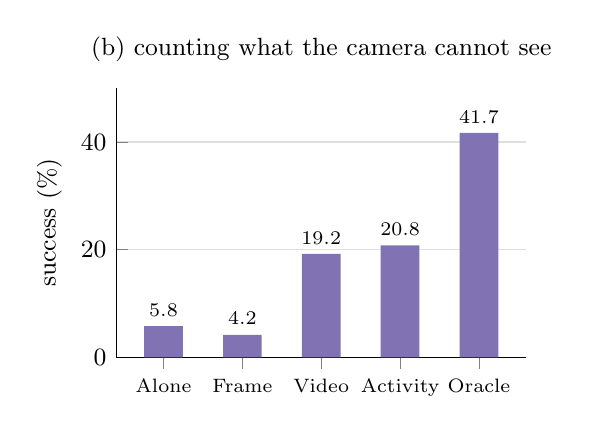
\begin{tikzpicture}
\begin{axis}[ybar, bar width=14pt, width=0.56\textwidth, height=5.0cm, ymax=50, ylabel={success (\%)}, enlarge x limits=0.15,
  symbolic x coords={Alone,Frame,Video,Activity,Oracle}, xtick=data, x tick label style={font=\scriptsize}, title={\small (b) counting what the camera cannot see}]
\addplot[fill=cE, draw=none] coordinates {(Alone,5.8) (Frame,4.2) (Video,19.2) (Activity,20.8) (Oracle,41.7)};
\end{axis}
\end{tikzpicture}
\caption{(a) An external memory re-issues a lost instruction. (b) ``Do it N times'' tasks where every repetition looks the same; \emph{Frame}: counting from the current image; \emph{Video}: learned video memory; \emph{Activity}: counting the robot's own grasp--lift--release cycles; \emph{Oracle}: perfect count.}
\label{fig:mem}
\end{figure}

\begin{figure}[!htbp]\centering
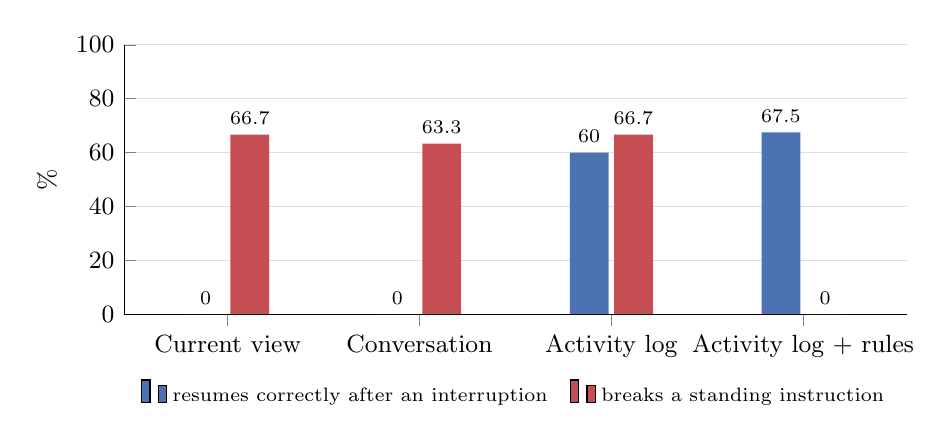
\begin{tikzpicture}
\begin{axis}[ybar, bar width=14pt, width=0.95\textwidth, height=5.0cm, ymax=100, ylabel={\%}, enlarge x limits=0.18,
  symbolic x coords={Current view,Conversation,Activity log,Activity log + rules}, xtick=data]
\addplot[fill=cA, draw=none] coordinates {(Current view,0) (Conversation,0) (Activity log,60) (Activity log + rules,67.5)};
\addplot[fill=cD, draw=none] coordinates {(Current view,66.7) (Conversation,63.3) (Activity log,66.7) (Activity log + rules,0)};
\legend{resumes correctly after an interruption, breaks a standing instruction}
\end{axis}
\end{tikzpicture}
\caption{What the planner remembers: ``First A, then B, then C'' $\rightarrow$ ``Wait, X first'' $\rightarrow$ ``OK, carry on'' (40 episodes), and ``Don't open any drawers today'' followed by other tasks (30 episodes). Planner: Qwen3-VL-4B.}
\label{fig:mem1}
\end{figure}

\sub{Results}
\begin{itemize}
\item \textbf{Lost instruction}: an external memory that re-issues the command raises success from 40\% to 86\%.
\item \textbf{Counting}: when every repetition looks the same, the robot alone succeeds 5.8\% of the time; a video memory reaches 19.2\% and a counter of its own grasp--lift--release cycles 20.8\% (a perfect count gives 41.7\%).
\item \textbf{Interruptions}: only the activity log lets the planner resume at the right step (60\%; the conversation alone or the current view: 0\%).
\item \textbf{Standing instructions}: stored as rules that remove forbidden skills, violations drop from 20/30 to 0/30. Kept only in the conversation, they are ignored.
\item \textbf{Full missions}: without memory, step-1 completion drops from 17/24 to 6/24.
\end{itemize}

\begin{table}[!htbp]\centering\small
\begin{tabularx}{\textwidth}{P{3.6cm}P{3.4cm}YP{1.6cm}}
\toprule
Memory & Solves & Result & Cost \\
\midrule
\textbf{Activity log} (plan, skills done, time per skill, interruptions) & resuming after an interruption & 23--27/40 vs 0--7/40, two planners & none \\
\textbf{Rules memory} & standing instructions & 20/30 $\rightarrow$ 0/30 violations & none \\
\textbf{Activity counter} (finger and hand sensors) & counts the camera cannot see & 20.8\% vs 5.8\% & none \\
Video memory (learned) & visual state over time & 19.2\%; next step right 74\% vs 54\% when scenes repeat & small model \\
Progress monitor with stop & ending multi-step tasks cleanly & 2/40 $\rightarrow$ 18--19/40 & small model \\
\bottomrule
\end{tabularx}
\caption{Memory types tested.}
\label{tab:mem}
\end{table}

\sub{Insights}
\begin{itemize}
\item The motion expert only sees the present; memory sits outside it and feeds the planner, so it works with any motion expert.
\item Cheap structured memories (activity log, rules, counters) cover most needs; a learned video memory helps where the scene hides progress.
\end{itemize}

\sub{What the literature shows}
LIBERO-Mem~\cite{liberomem} and MIKASA-Robo-VLA~\cite{mikasa} show that VLAs acting on the present frame fail tasks that need history. 3D-Mem~\cite{3dmem} keeps snapshots of key events for embodied reasoning.

%==================================================================
\section{Planner}
\label{sec:plan}
\begin{figure}[!htbp]\centering
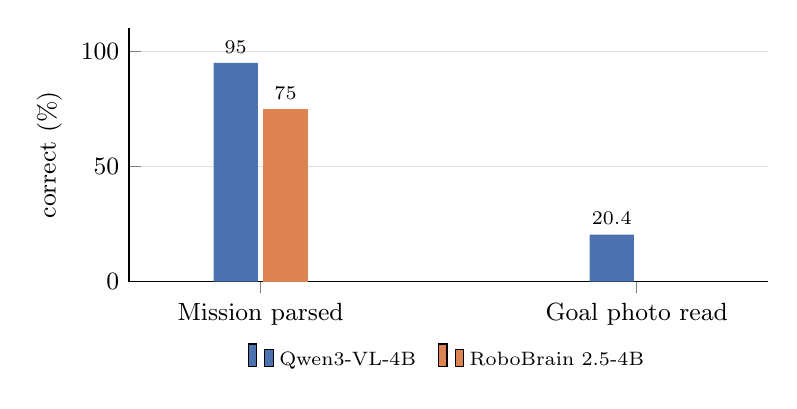
\begin{tikzpicture}
\begin{axis}[ybar, bar width=16pt, width=0.80\textwidth, height=4.8cm, ymax=110, ylabel={correct (\%)}, enlarge x limits=0.35,
  symbolic x coords={Mission parsed,Goal photo read}, xtick=data]
\addplot[fill=cA, draw=none] coordinates {(Mission parsed,95) (Goal photo read,20.4)};
\addplot[fill=cB, draw=none] coordinates {(Mission parsed,75)};
\legend{Qwen3-VL-4B, RoboBrain 2.5-4B}
\end{axis}
\end{tikzpicture}
\caption{Two 4B planners on the kitchen missions: turning the spoken mission into skills (80 missions) and reading a goal photo (Qwen3-VL-4B, 54 missions).}
\label{fig:plan}
\end{figure}

\sub{Results}
\begin{itemize}
\item Qwen3-VL-4B parses 76/80 spoken missions, RoboBrain 2.5-4B 60/80.
\item Goal photos are read poorly (11/54); the subtask-level world model reads them (\S\ref{sec:wm}).
\item Standing instructions kept in the conversation are ignored; rules memory handles them (\S\ref{sec:mem}).
\item Free-text sub-goals outside the motion expert's training vocabulary do not help (2/32 vs 4/32 on RoboCasa365).
\end{itemize}

\sub{Insights}
\begin{itemize}
\item Qwen3-VL-4B is the better base planner.
\item The planner works best when paired with the world model for pictures, rules memory for constraints, and sub-goals the motion expert knows.
\end{itemize}

\sub{What the literature shows}
Embodied VLMs such as RoboBrain~2.0~\cite{robobrain} and general VLMs such as Qwen3-VL~\cite{qwen3vl} decompose instructions and point at targets. \pzf~\cite{pi05} and \pzs~\cite{pi07} drive their action expert with subtasks from a high level.

%==================================================================
\section{Lessons for training}
\label{sec:lessons}
\begin{itemize}
\item \textbf{Own rollouts alone cause drift}: one fine-tuning round on its own rollouts made G0.5 11\% slower; mixing about 50\% original demonstrations into each round removed the drift.
\item \textbf{The noise is the safe place to improve}: the same learned critic that trained a useful noise policy broke the expert when applied to its weights.
\item \textbf{Modules outside the expert are independent of it}: memory, planner, world model and steering keep working when the expert changes.
\end{itemize}

\sub{What the literature shows}
Pretrained VLAs keep their skills over repeated fine-tuning~\cite{vla_forget}. A recent two-arm household study~\cite{agibot} scaled from 1,500 hours of demonstrations to corrections collected while the robot works.

%==================================================================
\parttitle{Part II \quad Proposal}

\section{Architecture}
\label{sec:arch}
\begin{center}
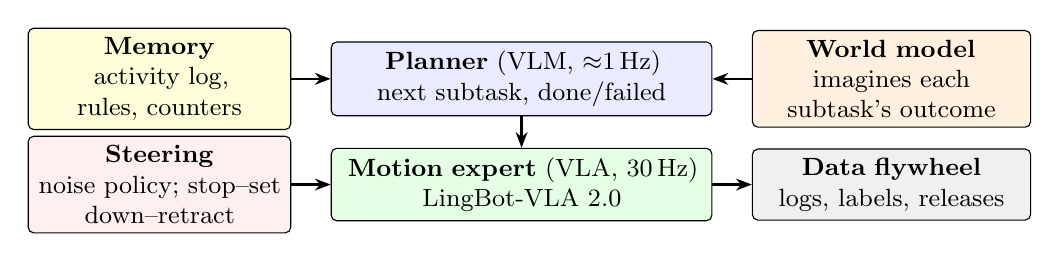
\begin{tikzpicture}[font=\small, node distance=4mm and 5mm,
  box/.style={draw, rounded corners=2pt, align=center, minimum height=8mm, fill=#1},
  arr/.style={-{Stealth[length=2mm]}, thick}]
\node[box=blue!8, text width=4.6cm] (plan) {\textbf{Planner} (VLM, $\approx$1\,Hz)\\next subtask, done/failed};
\node[box=yellow!15, left=of plan, text width=3.1cm] (mem) {\textbf{Memory}\\activity log, rules, counters};
\node[box=orange!12, right=of plan, text width=3.3cm] (wm) {\textbf{World model}\\imagines each subtask's outcome};
\node[box=green!10, below=of plan, text width=4.6cm] (vla) {\textbf{Motion expert} (VLA, 30\,Hz)\\LingBot-VLA 2.0};
\node[box=red!6, left=of vla, text width=3.1cm] (steer) {\textbf{Steering}\\noise policy; stop--set down--retract};
\node[box=gray!12, right=of vla, text width=3.3cm] (data) {\textbf{Data flywheel}\\logs, labels, releases};
\draw[arr] (mem) -- (plan); \draw[arr] (wm) -- (plan); \draw[arr] (plan) -- (vla); \draw[arr] (steer) -- (vla); \draw[arr] (vla) -- (data);
\end{tikzpicture}
\end{center}
The planner turns requests into short subtasks, using memory and the world model; the motion expert executes each subtask; the steering module redirects it when the user changes their mind; every run feeds the data flywheel.

%==================================================================
\section{Motion expert: LingBot-VLA 2.0}
\label{sec:prop-vla}
\sub{What LingBot brings}
\begin{itemize}
\item \textbf{Apache-2.0 licence}: free to use, modify and ship in a commercial product.
\item \textbf{Two arms, many robots}: one 55-dimensional action space with slots for arms, grippers, base and waist. OpenArm~2 maps onto slots the model already learned in pretraining.
\item \textbf{Richer perception}: short video input and a depth teacher during training, which helps grasping and contact.
\item \textbf{Runs on the robot}: $\approx$130\,ms per action chunk on one RTX 4090D.
\item \textbf{Same family as G0.5} (flow matching, 10-step sampler): the steering methods of Part~I apply directly.
\end{itemize}

\begin{table}[!htbp]\centering\small
\begin{tabularx}{\textwidth}{P{2.4cm}YYY}
\toprule
& \textbf{G0.5} & \textbf{LingBot-VLA 2.0} & \pzf\ / GR00T N1.7 \\
\midrule
Size, backbone & Qwen3.5 VLM + 635M action expert & 6B, Qwen3-VL-4B & 3B each \\
Robot bodies & single arm (LIBERO checkpoint) & two arms, base, waist; many robots & multi-robot; GR00T has an OpenArm~2 checkpoint \\
Perception & camera frames & camera frames + video, depth-trained & camera frames \\
\bottomrule
\end{tabularx}
\caption{Motion-expert candidates.}
\end{table}

\sub{Plan}
\begin{itemize}
\item \textbf{Simulation comparison}: LingBot, \pzf\ and GR00T trained on RoboCasa365 with the same budget, evaluated with the same harness.
\item \textbf{Bake-off on the OpenArm~2 data}: the three policies trained on our recordings, 10 tasks $\times$ 20 trials each on the robot.
\end{itemize}

\sub{What it means for the real robot}
A single consumer GPU on the robot runs LingBot in real time. Two-arm control and depth-aware perception match OpenArm~2 and household objects, and the licence lets the product ship.

\sub{What the literature shows}
LingBot-VLA 2.0~\cite{lingbot2} is a 6B model with a cross-embodiment action space, trained for two-arm robots. GR00T N1.7~\cite{gr00t} has an OpenArm~2 checkpoint.

%==================================================================
\section{Steering module}
\label{sec:prop-steer}
\begin{itemize}
\item \textbf{Noise policy as the learned steering module}, trained per skill from the robot's own rollouts.
\item \textbf{Stop, set down, retract, re-command} as the fallback.
\item \textbf{Retraction as teacher}: a student network learns from both cameras and the robot state how far the robot needs to back off in each situation, from not at all to a full retraction, to keep the fallback's reliability with less detour.
\item \textbf{Style preferences} through the same interface (PrefPI).
\end{itemize}

\sub{What it means for the real robot}
Users correct robots all the time. The noise policy needs no pointing and adds little latency. It is refreshed per skill from the robot's logs while the motion expert stays the same, and the retraction catches the cases it misses.

%==================================================================
\section{World model in the pipeline}
\label{sec:prop-wm}
\begin{figure}[!htbp]\centering
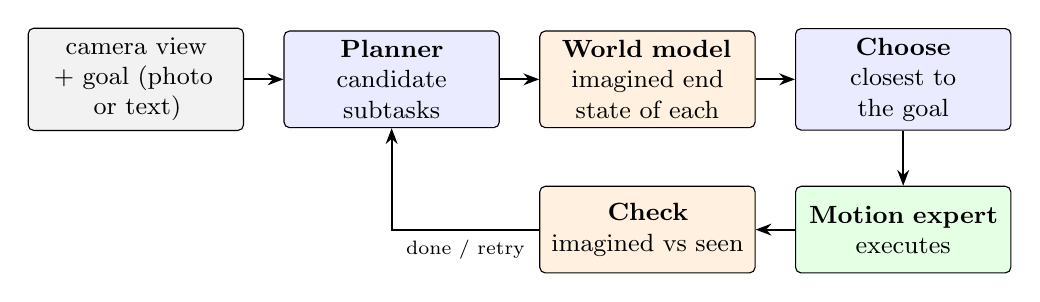
\begin{tikzpicture}[font=\small, node distance=4mm and 5mm,
  b/.style={draw, rounded corners=2pt, align=center, fill=#1, minimum height=11mm, text width=2.5cm},
  arr/.style={-{Stealth[length=2mm]}, thick}]
\node[b=gray!10] (in) {camera view\\+ goal (photo or text)};
\node[b=blue!8, right=of in] (pl) {\textbf{Planner}\\candidate subtasks};
\node[b=orange!12, right=of pl] (wm) {\textbf{World model}\\imagined end state of each};
\node[b=blue!8, right=of wm] (ch) {\textbf{Choose}\\closest to the goal};
\node[b=green!10, below=7mm of ch] (ex) {\textbf{Motion expert}\\executes};
\node[b=orange!12, left=of ex] (ck) {\textbf{Check}\\imagined vs seen};
\draw[arr] (in) -- (pl); \draw[arr] (pl) -- (wm); \draw[arr] (wm) -- (ch); \draw[arr] (ch) -- (ex); \draw[arr] (ex) -- (ck);
\draw[arr] (ck.west) -| node[pos=0.25, below, font=\scriptsize]{done / retry} (pl.south);
\end{tikzpicture}
\caption{The world model beside the planner.}
\end{figure}

\sub{What it adds}
\begin{enumerate}
\item \textbf{Picture goals}: ``make it look like this'' becomes a sequence of subtasks.
\item \textbf{Plan checking}: imagine a plan's outcome before running it.
\item \textbf{Success detection}: compare the imagined end state with the camera view; a mismatch triggers a retry or a question to the user.
\item \textbf{Training signal}: the critic and dynamics model behind the noise policies.
\item \textbf{Data curation}: score and filter logged episodes.
\end{enumerate}

\sub{What it means for the real robot}
A user can show a photo (``set the table like this''). The robot predicts the outcome of each subtask and checks it after doing it, which is the basis for success detection and later for safety checks. The model is small, ours, and trained on the robot's logs.

%==================================================================
\section{Memory}
\label{sec:prop-mem}
\begin{itemize}
\item \textbf{Activity log}: plan, skills done, time per skill, interruptions; read by the planner to resume.
\item \textbf{Rules memory}: standing instructions stored as forbidden skills.
\item \textbf{Activity counter}: repetitions counted from the robot's own finger and hand sensors.
\item \textbf{Video memory}: for tasks where the scene hides progress.
\item \textbf{Progress monitor}: issues the next step and stops the robot when the task is done.
\end{itemize}

\sub{What it means for the real robot}
Household work is interrupted, comes with standing preferences (``never put knives in that drawer'') and involves counts (three scoops, five shirts). The activity log, rules and counters cost nothing to run.

%==================================================================
\section{Planner}
\label{sec:prop-plan}
Qwen3-VL-4B is the baseline. Options to evaluate on the same missions:
{\small
\begin{xltabular}{\textwidth}{P{4.6cm}YP{3.0cm}}
\toprule
Option & What it brings & Cost \\
\midrule
\endfirsthead
\toprule
Option & What it brings & Cost \\
\midrule
\endhead
Qwen3-VL-4B fine-tuned (LoRA) on OpenArm subtask annotations and corrected plans & knowledge of our tasks and robot & $\approx$50--100 H200-h \\
Larger open VLMs (8B--32B) & better reasoning on long or vague requests & latency, GPU on the robot \\
Cloud models & strongest reasoning & latency, cost, privacy \\
Skill-vocabulary outputs (choose among the expert's trained subtasks) & no sub-goals the expert cannot execute & list of skills \\
Planner + subtask-level world model & picture goals, plan checks, success detection & small model \\
\bottomrule
\end{xltabular}}

\sub{What it means for the real robot}
The planner turns everyday speech into subtasks and handles corrections. It was the most frequent failure point in our missions, so improving it raises the reliability of the whole system.

%==================================================================
\section{Data and end-to-end training}
\label{sec:data}
\begin{table}[!htbp]\centering\small
\begin{tabularx}{\textwidth}{P{2.6cm}YP{3.2cm}P{3.0cm}}
\toprule
Module & Data & Labels & Scale in our runs \\
\midrule
Motion expert & teleoperated OpenArm~2 demonstrations cut into 2--10\,s subtasks; varied start states; \textbf{correction episodes} (operator takes over, then hands back) & subtask text (VLM proposal, checked by a person); success & 50 demonstrations per task (LIBERO) \\
Noise policy & robot rollouts with mid-task changes of instruction; retraction rollouts & success of the new subtask & 600--1,400 episodes \\
World model and critic & all logs, failures included: (view, subtask $\rightarrow$ end view) pairs; video and actions & automatic from logs & 382 demonstrations for 10 commands \\
Memory & event timelines; interruption and rule scenarios; repetition tasks & automatic from logs; scripted scenarios & 100 demonstrations per task \\
Planner & subtask annotations, corrected plans, goal photos & VLM proposals checked by a person & -- \\
Style preferences & rollouts ranked by an operator & rankings & $\approx$150 labels per preference (PrefPI) \\
\bottomrule
\end{tabularx}
\caption{Data per module. One recording session feeds several modules.}
\label{tab:data}
\end{table}

\begin{figure}[!htbp]\centering
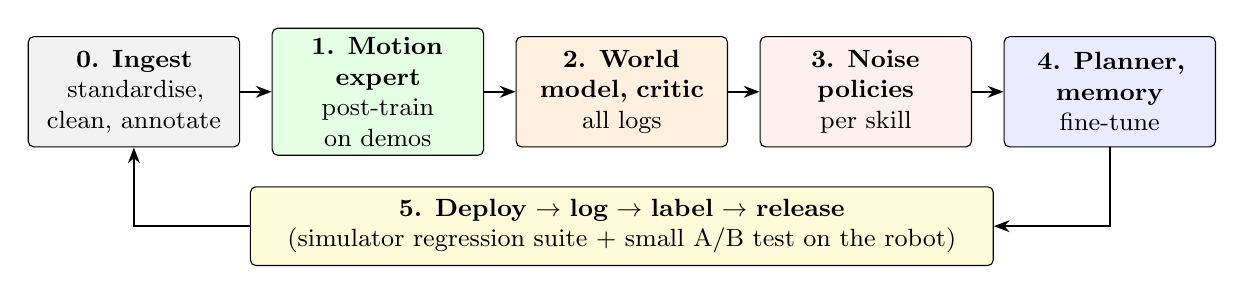
\begin{tikzpicture}[font=\small, node distance=4mm and 4mm,
  st/.style={draw, rounded corners=2pt, align=center, fill=#1, minimum height=14mm, text width=2.45cm},
  arr/.style={-{Stealth[length=2mm]}, thick}]
\node[st=gray!10] (s0) {\textbf{0. Ingest}\\standardise, clean, annotate};
\node[st=green!10, right=of s0] (s1) {\textbf{1. Motion expert}\\post-train on demos};
\node[st=orange!12, right=of s1] (s2) {\textbf{2. World model, critic}\\all logs};
\node[st=red!6, right=of s2] (s3) {\textbf{3. Noise policies}\\per skill};
\node[st=blue!8, right=of s3] (s4) {\textbf{4. Planner, memory}\\fine-tune};
\node[st=yellow!15, below=12mm of $(s1)!0.5!(s3)$, text width=9.2cm, minimum height=10mm] (s5) {\textbf{5. Deploy $\rightarrow$ log $\rightarrow$ label $\rightarrow$ release}\\(simulator regression suite + small A/B test on the robot)};
\draw[arr] (s0) -- (s1); \draw[arr] (s1) -- (s2); \draw[arr] (s2) -- (s3); \draw[arr] (s3) -- (s4);
\draw[arr] (s4.south) |- (s5.east); \draw[arr] (s5.west) -| (s0.south);
\end{tikzpicture}
\caption{The training flywheel.}
\label{fig:fly}
\end{figure}

\sub{Training stages}
\begin{enumerate}
\setcounter{enumi}{-1}
\item \textbf{Ingest}: one control rate, camera names, joint order and gripper convention; broken episodes removed; episodes split into subtasks with language.
\item \textbf{Motion expert}: post-train LingBot on the OpenArm demonstrations, correction episodes included, with original demonstrations mixed into every later round.
\item \textbf{World model and critic}: trained on all logs, failures included.
\item \textbf{Noise policies}: per skill, imitate successful noises, then improve through the world model and critic.
\item \textbf{Planner and memory}: fine-tune the planner on annotated subtasks and corrected plans; build memories from event timelines.
\item \textbf{Deploy, log, label, release}: take-overs and success labels flow back into steps 0--4; a new version ships after the simulator regression suite and a small A/B test on the robot.
\end{enumerate}

\begin{table}[!htbp]\centering\small
\begin{tabularx}{\textwidth}{YP{3.6cm}}
\toprule
Stage & Compute \\
\midrule
Motion-expert comparison (RoboCasa365) and bake-off on OpenArm data & 600--1,000 H200-h \\
World model and critic on OpenArm data & 100--200 H200-h \\
Planner fine-tune (Qwen3-VL-4B, LoRA) & 50--100 H200-h \\
Noise policies, memory modules, evaluation & $\approx$400 T4-h \\
\bottomrule
\end{tabularx}
\caption{Compute per stage.}
\end{table}

\sub{What it means for the real robot}
Every hour of operation produces training data for all modules: operator take-overs become correction data, failures train the world model and critic, and each release is tested before it ships.

\section*{Requests}
\begin{enumerate}
\item \textbf{Compute}: $\approx$600--1,000 H200-hours for the motion-expert comparison, $\approx$100--200 for the world model and critic, $\approx$50--100 for the planner fine-tune.
\item \textbf{Data}: access to the OpenArm~2 recordings.
\end{enumerate}

\begin{thebibliography}{99}\small
\bibitem{pi05} K.~Black et al. \pzf: a vision-language-action model with open-world generalization. CoRL (PMLR 305), 2025.
\bibitem{pi07} Physical Intelligence. \pzs. arXiv:2604.15483, 2026.
\bibitem{g05} Galaxea. G0.5. arXiv:2608.11739, 2026. \url{https://github.com/OpenGalaxea/GalaxeaVLA}
\bibitem{awomo} Awomo-0.5. \url{https://github.com/Awomo-WestlakeDI/Awomo-0.5}
\bibitem{gr00t} NVIDIA. Isaac GR00T N1.7. \url{https://github.com/NVIDIA/Isaac-GR00T}
\bibitem{lingbot2} Robbyant. LingBot-VLA 2.0. 2026. \url{https://github.com/robbyant/lingbot-vla-v2}
\bibitem{vla_forget} Pretrained vision-language-action models are surprisingly resistant to forgetting in continual learning. arXiv:2603.03818, 2026.
\bibitem{robojepa} RoboJEPA: Scaling robotic latent world models. arXiv:2610.10515, 2026.
\bibitem{lawam} LaWAM. arXiv:2606.15768, 2026.
\bibitem{flare} FLARE: Robot learning with implicit world modeling. arXiv:2505.15659, 2025.
\bibitem{cosmos3} NVIDIA. Cosmos 3. \url{https://huggingface.co/collections/nvidia/cosmos3}
\bibitem{flux3a} Black Forest Labs. FLUX 3 Action. \url{https://huggingface.co/black-forest-labs/flux-3-action-droid}
\bibitem{openwam} OpenWAM: An open, modular exploration towards systematic world-action model pretraining. arXiv:2609.07398, 2026.
\bibitem{dreamerv3} D.~Hafner et al. Mastering diverse domains through world models (DreamerV3). 2023.
\bibitem{tdmpc2} N.~Hansen et al. TD-MPC2: Scalable, robust world models for continuous control. ICLR, 2024.
\bibitem{supermimic} Q.~Liao et al. SuperMimic: Scaling humanoid whole-body control with one differentiable world model. CoRL, 2026. arXiv:2610.28480.
\bibitem{cfg} J.~Ho, T.~Salimans. Classifier-free diffusion guidance. arXiv:2207.12598, 2022.
\bibitem{cfgrl} K.~Frans, S.~Park, P.~Abbeel, S.~Levine. Diffusion guidance is a controllable policy improvement operator. arXiv:2505.23458, 2025.
\bibitem{frs} Improving robotic generalist policies via flow reversal steering. arXiv:2606.13675, 2026.
\bibitem{dsrl} A.~Wagenmaker et al. Steering your diffusion policy with latent space reinforcement learning. CoRL, 2025.
\bibitem{flowdagger} FlowDAgger: Human-in-the-loop adaptation of generative robot policies in latent space. arXiv:2607.08877, 2026.
\bibitem{prefpi} S.~Rho, W.~Kim, D.~Xu, S.~Ha. PrefPI: Preference-guided steering into out-of-distribution behaviors. arXiv:2609.40165, 2026.
\bibitem{liberomem} Chung et al. LIBERO-Mem. arXiv:2511.11478, 2025.
\bibitem{mikasa} MIKASA-Robo-VLA: Benchmarking memory in VLA models for long-horizon manipulation. arXiv:2610.00604, 2026.
\bibitem{3dmem} 3D-Mem: 3D scene memory for embodied exploration and reasoning. CVPR, 2025. arXiv:2411.17735.
\bibitem{robobrain} BAAI. RoboBrain 2.0 technical report. arXiv:2507.02029, 2025.
\bibitem{qwen3vl} Qwen Team. Qwen3-VL. 2025.
\bibitem{robocasa365} RoboCasa365: A large-scale simulation framework for training and benchmarking generalist robots. arXiv:2603.04356, 2026.
\bibitem{agibot} Scaling bimanual household manipulation from 1,500 hours of demonstrations to on-policy corrections. arXiv:2609.03591, 2026.
\end{thebibliography}
\end{document}
